\section{Replicate Ordering\label{sec:app1:ordering}}

This enhancement is based on replicate ordering and is similar to the port-ordering modification that the original tree algorithm is based on \cite{Herber2017a}. Now, we eliminate some component-type isomorphisms during the graph generation process.

\subsection{Theory}
Consider a single component type and its set of $N$ replicates.
Now, consider a single replicate numbered $n$ and $n\neq 1$.
During an iteration of the tree algorithm (Alg.~\ref{alg:app1:tree}), a single edge is added.
If replicate $n-1$ still has no ports connected, then adding this edge to $n$ will produce a graph isomorphic to the graph created when adding the edge to $n-1$.
This claim is based on the component-type isomorphism issue where we have two identical replicates currently with no edges.
Therefore, we only need to allow a connection to $n-1$ and not to $n$, and the tree algorithm will continue generating the desired graph structure space.
When $n=1$, an edge will always be allowed since there is no other replicate to compare against.

This enhancement is general since it does not rely on any \glsfirstplural[noindex]{NSC} being present.

\subsection{Implementation}

\begin{vAlgorithm}[!ht]{\columnwidth}{0em}
\LinesNumbered
\DontPrintSemicolon

\SetKwFunction{circshift}{circshift}

\SetKwInOut{Input}{Input}
\SetKwInOut{Output}{Output}

\caption{Limit potential connections based on replicate ordering.\label{alg:app1:ordering}}

\Input{%
        \xvbox{2.5mm}{$\xvar{V}$} -- vector of remaining ports for each component replicate \\
        \xvbox{2.5mm}{$\xvar{Vf}$} -- initial vector of ports available for each component replicate \\
        $\xvar{iInitRep}$ -- indices of the initial replicate for each component type
      }
\Output{%
        $\xvar{Vordering}$ -- binary vector where $1$ indicates an edge is possible, $0$ if it is not
       }

\BlankLine

$\xvar{Vordering}$ $\leftarrow$ $\circshift(\xvar{V},[1])$ $\neq$ $\xvar{Vf}$ \tcc*{check if left neighbor has a connection\label{alg:app1:ordering-l1}}

$\xvar{Vordering}(\xvar{iInitRep})$ $\leftarrow$ 1 \tcc*{initial replicates are always 1\label{alg:app1:ordering-l2}}

\end{vAlgorithm}

Algorithm~\ref{alg:app1:ordering} is the pseudocode for the implementation of this enhancement.
The implementation is centered around the creation of a binary vector ($\xvar{Vordering}$) with length equal to the total number of components where unity indicates a connection is allowed and zero indicates it is not. 
This enhancement is implemented efficiently with the $\texttt{circshift}(v,k)$ function.
This function circularly shifts the elements in array $v$ by $k$ positions \cite{matlab-circshift}.
Based on the discussion above, we want to determine if $n-1$ has been connected to any other vertex.
Using the initial vector of ports available for each component replicate ($\xvar{Vf}$), we \texttt{circshift} the vector of remaining ports for each component replicate ($\xvar{V}$) by one position to the right and compare these vectors (see line~\ref{alg:app1:ordering-l1}). 
A pair that is not equal indicates $n-1$ has at least one edge, so we now need to allow connections to $n$.

The procedure above will produce incorrect results for the initial replicates. However, we have that these initial replicates should never have their connection disallowed so we simply ensure that their index in $\xvar{Vordering}$ is always unity (see line~\ref{alg:app1:ordering-l2}).
The indices of the initial replicate for each component type ($\xvar{iInitRep}$) is calculated before the tree algorithm is called since it does not change throughout the graph generation procedure.

This enhancement is inserted between lines~\ref{alg:app1:tree-rmport1} and \ref{alg:app1:tree-Vallow} of Alg.~\ref{alg:app1:tree} and line~\ref{alg:app1:tree-Vallow} is changed to:
\begin{align}
\xvar{Vallow} = \xvar{V} \ \gls{hadamard}\ \xvar{A(iL,:)} \circ \xvar{Vordering} 
\end{align}

\noindent Now, $\xvar{Vordering}$ can disallow connections in the same way as $\xvar{A(iL,:)}$.

\subsection{Examples}

\subsubsection{Example 1\label{sec:app1:ordering-ex1}}

The base three-tuple and NSCs for this example are specified as:
\begin{align}
C = \{ \xcolor{X} \}, \quad R = [4], \quad P = [2], \quad \text{no additional NSCs}
\end{align}

\noindent The second and third inputs for Algorithm~\ref{alg:app1:ordering} are:
\begin{align}
\xvar{Vf} = \text{[2 2 2 2]}, \quad \xvar{iInitRep} = [1]
\end{align}

We will consider two different $\xvar{V}$, one at the initial iteration of the tree algorithm and one at some intermediate iteration.
Figure~\ref{tb:app1:ordering-ex1-V} goes through the operations in Algorithm~\ref{alg:app1:ordering} for the different $\xvar{V}$.
The example iterations are also visualized in Figs.~\ref{fig:app1:ordering-ex1-original} and \ref{fig:app1:ordering-ex1-intermediate}.

Table~\ref{tb:app1:ordering-ex1} compares the original algorithm with the enhancement for this example.
There is a reduction in candidate graphs generated while the number of unique graphs remains the same.

\begin{figure}[!ht]

\begin{subfigure}[b]{\textwidth}
\centering
\begin{tabular}{r | c | c}
\hline \hline
 & Initial & Intermediate \\ 
\hline
$\xvar{V}$ & [1 2 2 2] & [0 0 1 2] \\
$\texttt{circshift}(\xvar{V} [0\ 1])$  & [2 1 2 2] & [2 0 0 1] \\
$\xvar{Vf}$  & [2 2 2 2] & [2 2 2 2] \\
$\circshift(\xvar{V}[0\ 1]) \neq \xvar{Vf}$  & [0 1 0 0] & [0 1 1 1] \\
$\xvar{Vordering}(\xvar{iInitRep}) \leftarrow 1$ & [1 1 0 0] & [1 1 1 1] \\
Removed/total branches & 2/4 & 0/2 \\
\hline \hline
\end{tabular}
\caption{Algorithm operations.\label{tb:app1:ordering-ex1-V}}
\end{subfigure}%

\begin{subfigure}[b]{0.5\textwidth}
\centering
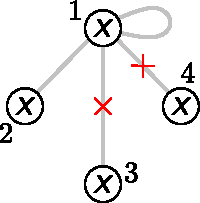
\includegraphics[scale=1]{../app1/fig/ordering-ex1-original_v2}
\caption{Initial iteration.\label{fig:app1:ordering-ex1-original}}
\end{subfigure}%
\begin{subfigure}[b]{0.5\textwidth}
\centering
 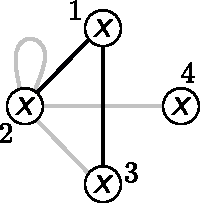
\includegraphics[scale=1]{../app1/fig/ordering-ex1-intermediate_v2}
 \caption{Intermediate iteration.\label{fig:app1:ordering-ex1-intermediate}}
\end{subfigure}%

\caption{\nameref{sec:app1:ordering-ex1} for Algorithm~\ref{alg:app1:ordering} (replicate ordering).}
\end{figure}

\begin{table}[!ht]
\centering
\caption{Comparison (replicate ordering, \nameref{sec:app1:ordering-ex1}). \label{tb:app1:ordering-ex1}}
\begin{tabular}{r | c | c | c}
\hline \hline
& Orig & En & Orig/En \\
\hline
Candidate Graphs & 26 & 8 & 3.25 \\
Unique Graphs & 5 & 5 & 1 \\
Generation Time (s) & 0.0052 & 0.0033 & 1.58 \\
Total Time (s) & 0.0095 & 0.0060 & 1.58 \\
\hline \hline
\end{tabular}
\end{table}

\subsubsection{Example 2\label{sec:app1:ordering-ex2}}

The base three-tuple and NSCs for this example are specified as:
\begin{align}
C = \{ \xcolor{W}, \xcolor{X}, \xcolor{Y}, \xcolor{Z}\}, \quad R = [3\ 4\ 2\ 1], \quad P = [1\ 2\ 2\ 3], \quad \text{no additional NSCs}
\end{align}

\noindent The second and third inputs for Algorithm~\ref{alg:app1:ordering} are:
\begin{align}
\xvar{Vf} = \text{[1 1 1 2 2 2 2 2 2 3]}, \quad \xvar{iInitRep} = \text{[1 4 8 10]}
\end{align}

We will consider two different $\xvar{V}$, one at the initial iteration of the tree algorithm and one at some intermediate iteration. Figure~\ref{tb:app1:ordering-ex2-V} goes through the operations in Algorithm~\ref{alg:app1:ordering} for the different $\xvar{V}$.
The example iterations are also visualized in Figs.~\ref{fig:app1:ordering-ex2-original} and \ref{fig:app1:ordering-ex2-intermediate}.

Table~\ref{tb:app1:ordering-ex2} compares the original algorithm with the enhancement for this example. There is a reduction in candidate graphs generated while the number of unique graphs remains the same.

\begin{figure}[!ht]

\begin{subfigure}[b]{\textwidth}
\centering
\begin{tabular}{r | c | c}
\hline \hline
 & Initial & Intermediate \\ 
\hline
$\xvar{V}$ & [0 1 1 2 2 2 2 2 2 3] & [0 0 0 0 1 2 2 1 2 3] \\
$\texttt{circshift}(\xvar{V} [0\ 1])$  & [3 0 1 1 2 2 2 2 2 2] & [3 0 0 0 0 1 2 2 1 2] \\
$\xvar{Vf}$  & [1 1 1 2 2 2 2 2 2 3] & [1 1 1 2 2 2 2 2 2 3] \\
$\circshift(\xvar{V}[0\ 1]) \neq \xvar{Vf}$  & [1 1 0 1 0 0 0 0 0 1] & [1 1 1 1 1 1 0 0 1 1] \\
$\xvar{Vordering}(\xvar{iInitRep}) \leftarrow 1$ &  [1 1 0 1 0 0 0 1 0 1] & [1 1 1 1 1 1 0 1 1 1]  \\
Removed/total branches & 5/9 & 1/6 \\
\hline \hline
\end{tabular}
\caption{Algorithm operations.\label{tb:app1:ordering-ex2-V}}
\end{subfigure}%

\begin{subfigure}[b]{0.5\textwidth}
\centering
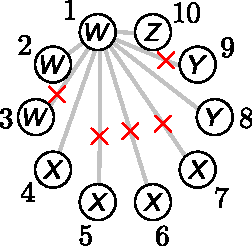
\includegraphics[scale=1]{../app1/fig/ordering-ex2-original_v2}
\caption{Initial iteration.\label{fig:app1:ordering-ex2-original}}
\end{subfigure}%
\begin{subfigure}[b]{0.5\textwidth}
\centering
 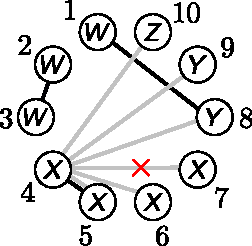
\includegraphics[scale=1]{../app1/fig/ordering-ex2-intermediate_v2}
 \caption{Intermediate iteration.\label{fig:app1:ordering-ex2-intermediate}}
\end{subfigure}%

\caption{\nameref{sec:app1:ordering-ex2} for Algorithm~\ref{alg:app1:ordering} (replicate ordering).}
\end{figure}

\begin{table}[!ht]
\centering
\caption{Comparison (replicate ordering, \nameref{sec:app1:ordering-ex2}).\label{tb:app1:ordering-ex2}}
\begin{tabular}{r | c | c | c}
\hline \hline
& Orig & En & Orig/En \\
\hline
Candidate Graphs & 456766 & 14359 & 31.8 \\
Unique Graphs & 1657 & 1657 & 1 \\
Generation Time (s) & 16.26 & 0.69 & 23.6 \\
Total Time (s) & 3577 & 145 & 24.7 \\
\hline \hline
\end{tabular}
\end{table}